% !TEX program = xelatex
\documentclass[11pt,a4paper]{ctexart}
\usepackage[margin=2.25cm]{geometry}
\usepackage{booktabs,graphicx,float,array,xcolor,longtable}
\usepackage[hidelinks]{hyperref}
\usepackage{caption}
\captionsetup{font=small,labelfont=bf}
\setlength{\parindent}{2em}
\setlength{\parskip}{0.35em}
\setlength{\tabcolsep}{5pt}
\newcommand{\SalesSeventeen}{303.0}
\newcommand{\SalesEighteen}{726.8}
\newcommand{\OrdersSeventeen}{22,137}
\newcommand{\OrdersEighteen}{52,934}
\newcommand{\SalesGrowth}{+139.8\%}
\newcommand{\OrderGrowth}{+139.1\%}
\newcommand{\AverageGrowth}{+0.3\%}
\newcommand{\MissingShareSeventeen}{1.6\%}
\newcommand{\MissingShareEighteen}{1.0\%}
\newcommand{\SmallBaseShare}{6.7\%}
\newcommand{\CommonRevenueShare}{99.9\%}
\newcommand{\StarCount}{32}
\newcommand{\StarSales}{325.7}
\newcommand{\StarShare}{44.8\%}
\newcommand{\StarSalesGrowth}{+267.0\%}
\newcommand{\StarOrderGrowth}{+281.5\%}
\newcommand{\CowCount}{4}
\newcommand{\CowSales}{54.6}
\newcommand{\CowShare}{7.5\%}
\newcommand{\CowSalesGrowth}{+126.4\%}
\newcommand{\CowOrderGrowth}{+183.5\%}
\newcommand{\PotentialCount}{3}
\newcommand{\PotentialSales}{60.4}
\newcommand{\PotentialShare}{8.3\%}
\newcommand{\PotentialSalesGrowth}{+198.3\%}
\newcommand{\PotentialOrderGrowth}{+120.0\%}
\newcommand{\DogCount}{30}
\newcommand{\DogSales}{285.5}
\newcommand{\DogShare}{39.3\%}
\newcommand{\DogSalesGrowth}{+68.0\%}
\newcommand{\DogOrderGrowth}{+72.4\%}


\title{\bfseries 电商二级品类经营矩阵分析\\[0.3em]
\large 2018 年 1—8 月与 2017 年同期对比}
\author{大数据案例实务分析课程作业}
\date{2026 年 9 月}

\begin{document}
\pagestyle{plain}
\maketitle

\begin{abstract}
本文比较 Olist 平台 2017 年与 2018 年 1—8 月的商品销售，
以品类销售额和订单量的同比增速建立四象限矩阵，并提出分类经营建议。
2018 年有品类信息的商品销售额为 \SalesEighteen{} 万 BRL，
同比 \SalesGrowth{}；涉及 \OrdersEighteen{} 笔订单，
同比 \OrderGrowth{}。69 个两期均有销售的品类中，
明星类占当年销售额的 \StarShare{}，瘦狗类仍占 \DogShare{}。
因此，资源配置既要考虑增长速度，也要考虑现有销售规模。
\end{abstract}

\begin{table}[H]
\centering
\caption{销售规模与品类分类概况}
\begin{tabular}{p{4.0cm}p{4.5cm}p{6.2cm}}
\toprule
指标 & 结果 & 说明 \\
\midrule
商品销售额 & \SalesEighteen{} 万 BRL（\SalesGrowth{}） & 2018 年有品类信息的商品金额及同比 \\
去重订单数 & \OrdersEighteen{} 单（\OrderGrowth{}） & 2018 年涉及上述商品的订单及同比 \\
明星品类销售额占比 & \StarShare{}（\StarCount{} 类） & 销售额、订单量增速均高于平台 \\
瘦狗品类销售额占比 & \DogShare{}（\DogCount{} 类） & 两项增速均低于平台，但销售规模较大 \\
\bottomrule
\end{tabular}
\end{table}

\section{数据与方法}

分析使用提供的 Olist 订单、订单明细、商品和品类翻译四张表。
根据订单表记录的下单时间，分别提取 2017 年和 2018 年
1 月 1 日至 8 月 31 日的订单，两期均为 243 天。保留
\texttt{approved}、\texttt{processing}、\texttt{invoiced}、
\texttt{shipped} 和 \texttt{delivered} 状态，排除仅创建、缺货和已取消的订单。
由于 2018 年 8 月的部分订单在数据截止时尚未送达，仅统计已送达订单会低估当期下单金额。

本文所称品类销售额为下单商品在订单明细中 \texttt{price} 的合计，
不含运费，也未扣除成本，不能等同于已确认收入；
品类订单量为购买该品类的去重 \texttt{order\_id} 数。
一笔订单涉及多个品类时，分别计入各品类的订单量，
因而各品类订单量之和可能超过平台去重订单数。

剔除品类信息缺失的商品后，2017 年和 2018 年的商品销售额分别为
\SalesSeventeen{}/\SalesEighteen{} 万 BRL，去重订单为
\OrdersSeventeen{}/\OrdersEighteen{} 单。缺失品类金额分别占同期有效订单
商品金额的 \MissingShareSeventeen{}/\MissingShareEighteen{}。
分析以原表的品类字段为单位，按作业要求称为二级品类。
两期均有销售的 69 类纳入矩阵；2018 年新增 3 类、退出 1 类，单独列示。

\begin{table}[H]
\centering
\caption{两期数据筛选结果}
\small
\begin{tabular}{lrr}
\toprule
统计项 & 2017 年 1—8 月 & 2018 年 1—8 月 \\
\midrule
有效订单数 & 22,562 & 53,530 \\
商品明细行数 & 25,576 & 61,135 \\
缺失品类明细行数 & 496 & 680 \\
有品类信息订单数 & 22,137 & 52,934 \\
有品类信息商品金额／万 BRL & 303.0 & 726.8 \\
\bottomrule

\end{tabular}
\end{table}
\noindent 有品类信息的订单数小于有效订单数，差额来自商品品类信息缺失。
订单号和商品号在各自主表中均不重复；分析脚本还检查了订单明细重复、
商品档案缺失、非正价格和金额汇总。

\subsection{指标计算与分类标准}

\begin{enumerate}
\item 按订单号连接订单与商品明细，按商品号连接商品档案，并用翻译表确定品类名称。
\item 按下单时间和订单状态筛选两期数据，单独记录品类信息缺失的商品。
\item 分别汇总每个品类的商品金额和去重订单数；仅对两期均有销售的品类计算同比。
\item 计算同期有品类信息商品的整体增速，以其为分界划分品类象限。2017 年不足 30 单的品类仍参与分类，在附录中单独标记。
\end{enumerate}

对品类 $c$，销售额同比 $g_R^c=R_{2018}^c/R_{2017}^c-1$，
订单量同比 $g_O^c=O_{2018}^c/O_{2017}^c-1$。
矩阵分别以\textbf{整体销售额同比 \SalesGrowth{} 和订单量同比 \OrderGrowth{}}
为横、纵轴分界。若以 0\% 为分界，69 类中有 54 类集中于双增长象限；
采用整体增速可进一步区分各品类的相对增长水平。
题目配图的纵轴标为“利润率”，但文字要求使用“订单量同比增长率”，
且原始数据缺少计算利润率所需的成本数据。因此，矩阵纵轴采用订单量同比，
象限位置及名称沿用配图。文中的“高”“低”仅表示相对于整体增速的比较结果。

\begin{table}[H]
\centering
\caption{四象限分类标准}
\small
\begin{tabular}{lp{3.3cm}p{3.3cm}p{6.5cm}}
\toprule
象限 & 销售额同比 & 订单量同比 & 数据特征及经营重点 \\
\midrule
明星 & 高于或等于整体 & 高于或等于整体 & 两项增速较高，保障供给并评估投放效率 \\
金牛 & 低于整体 & 高于或等于整体 & 订单增长较快，关注单均商品金额 \\
潜力 & 高于或等于整体 & 低于整体 & 销售额增长较快，争取更多订单 \\
瘦狗 & 低于整体 & 低于整体 & 两项增速较低，结合销售规模调整投入 \\
\bottomrule
\end{tabular}
\end{table}

\section{矩阵结果}

\begin{figure}[H]
\centering
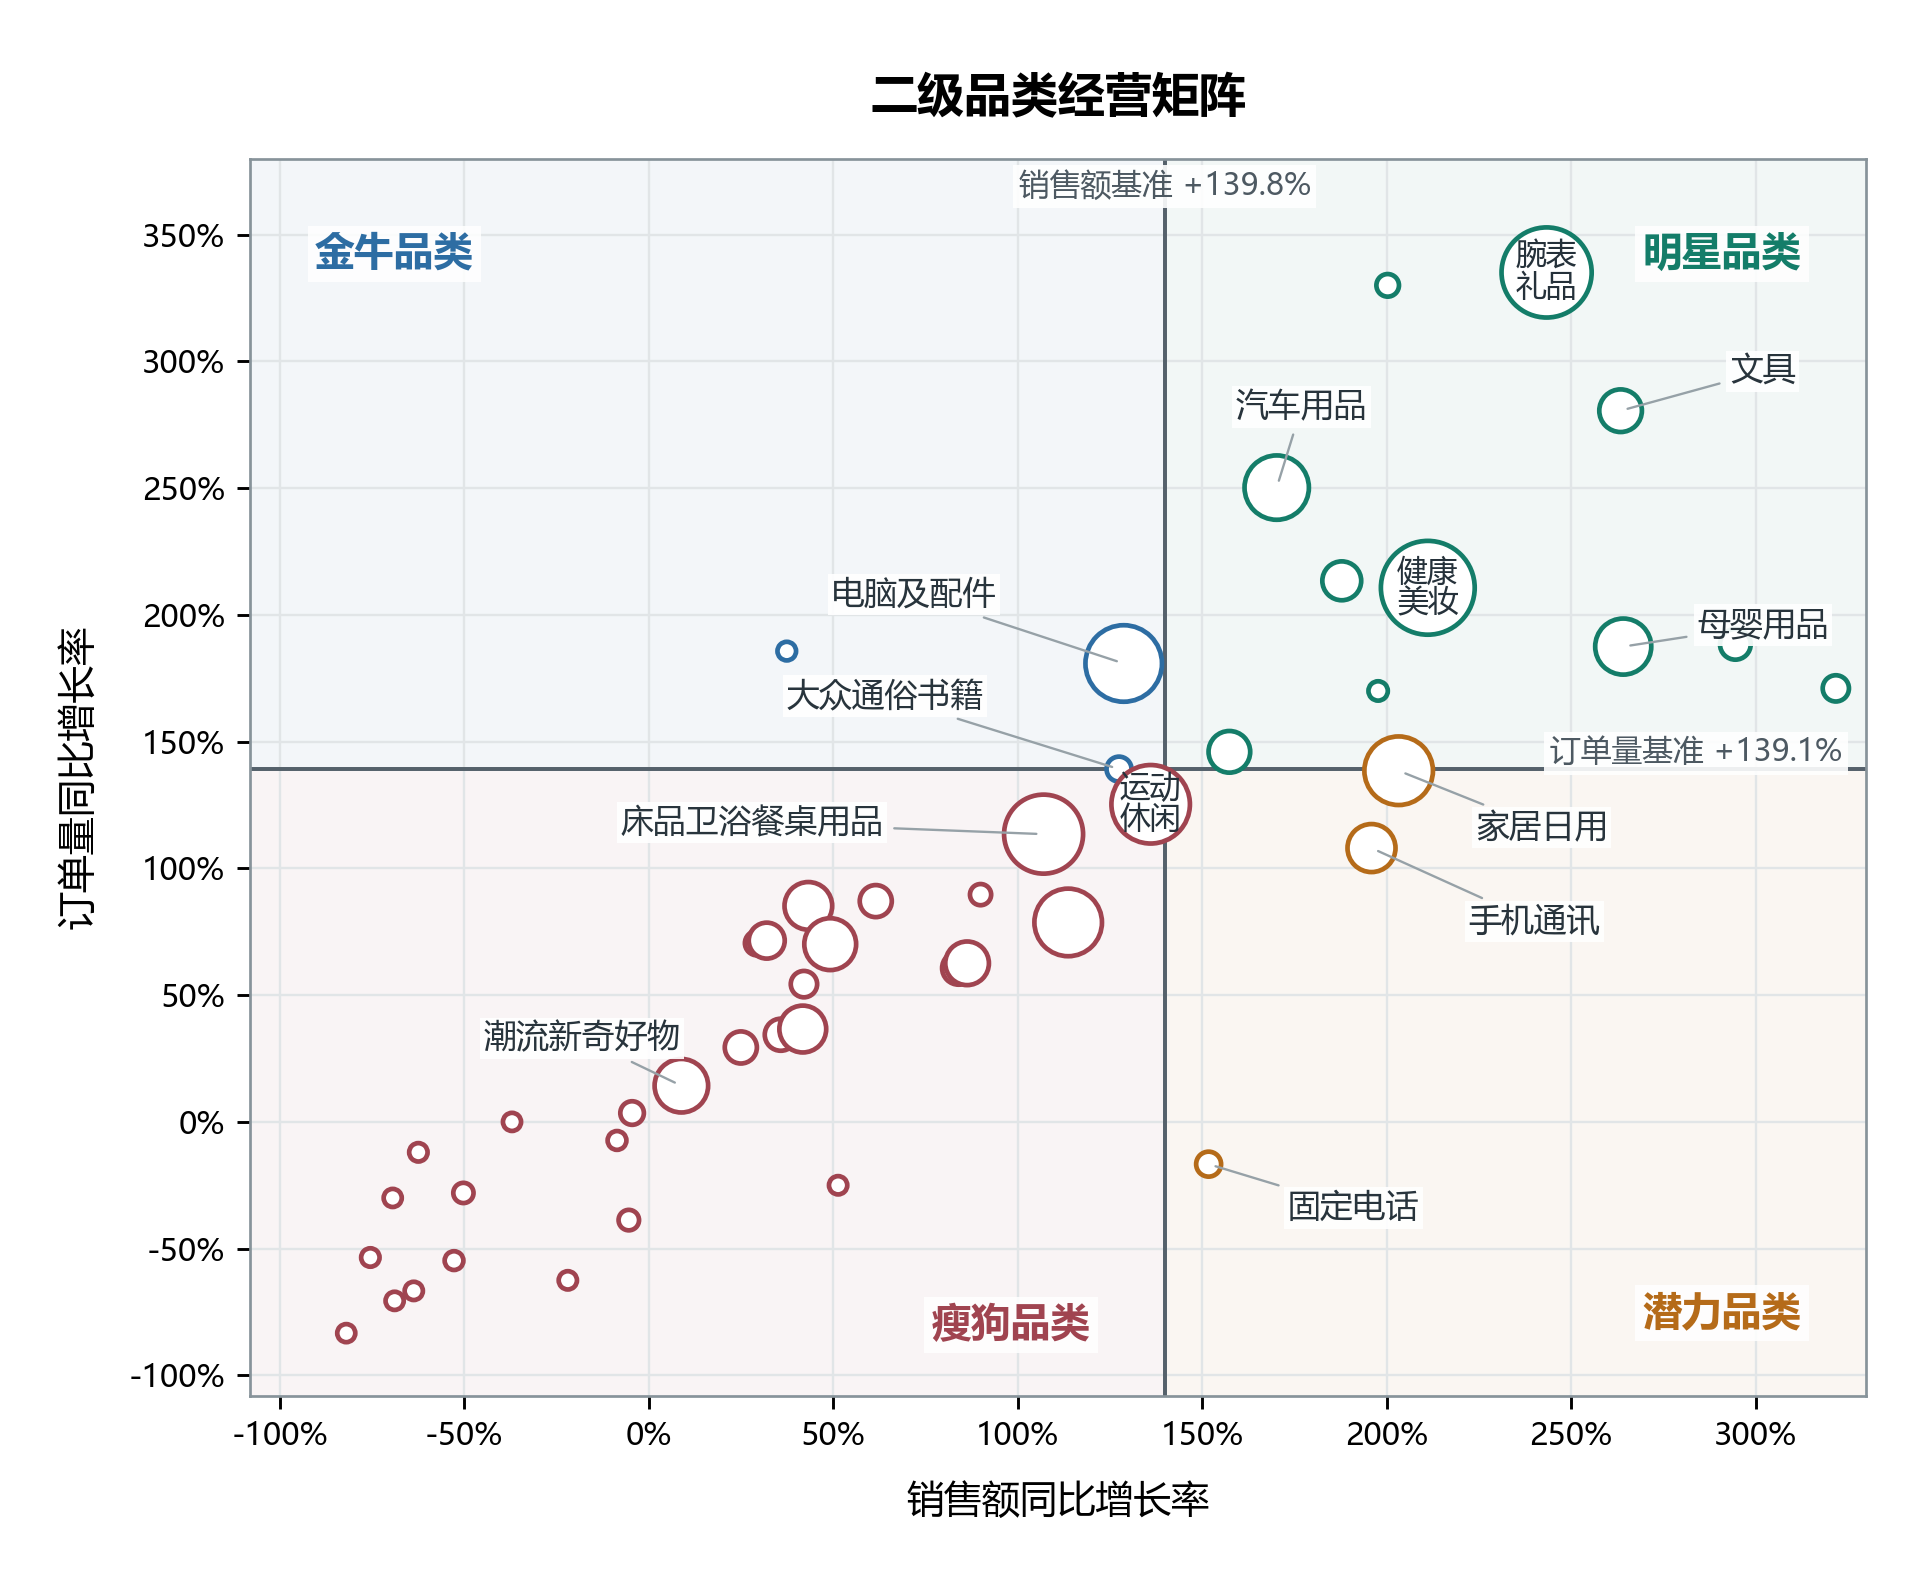
\includegraphics[width=\textwidth]{figures/matrix.png}
\caption{二级品类销售额与订单量同比矩阵。图内展示 47 类，
占可比品类 2018 年销售额的 90.2\%；圆圈越大，销售额越高。其余品类见附录。}
\end{figure}
\noindent 图内直接标出主要销售品类和分界线附近的品类。
下表按全部 69 类汇总分类结果。

\begin{table}[H]
\centering
\caption{四象限品类数与销售情况}
\footnotesize
\begin{tabular}{lrrrrrr}
\toprule
象限 & 品类数 & 2018 销售额\,/万 BRL & 销售额占比 & 销售同比 & 品类订单同比 & 低基数类数 \\
\midrule
明星 & 32 & 325.7 & 44.8\% & +267.0\% & +281.5\% & 17 \\
金牛 & 4 & 54.6 & 7.5\% & +126.4\% & +183.5\% & 2 \\
潜力 & 3 & 60.4 & 8.3\% & +198.3\% & +120.0\% & 0 \\
瘦狗 & 30 & 285.5 & 39.3\% & +68.0\% & +72.4\% & 9 \\
\bottomrule

\end{tabular}
\end{table}

\noindent 销售额占比以 2018 年有品类信息的商品销售额为分母；
四象限合计略低于 100\%，因为新增的 3 类未进入矩阵。
象限订单同比按品类订单数合计计算，跨品类订单可重复计入。

\section{分类结果与经营建议}

\noindent\textbf{明星品类。}
\StarCount{} 类，2018 年销售额 \StarSales{} 万 BRL、占 \StarShare{}；
销售额同比为 \StarSalesGrowth{}，品类订单同比为 \StarOrderGrowth{}，
均高于整体水平。
健康美妆销售额 77.0 万 BRL（销售同比 +211.2\%、订单 +210.7\%），
腕表礼品为 70.8 万 BRL（+243.4\%、+335.1\%）。
建议保障畅销商品库存与配送能力，并依据投放效果决定增量资源。
腕表礼品的订单增速高于销售额增速，单均商品金额约下降 21.1\%，
应结合商品结构和促销费用观察增长质量。

\noindent\textbf{金牛品类。}
\CowCount{} 类，销售额 \CowSales{} 万 BRL、占 \CowShare{}；
品类订单同比 \CowOrderGrowth{} 高于整体水平，而销售同比 \CowSalesGrowth{} 低于整体水平。
电脑及配件贡献 50.2 万 BRL，占金牛类销售额约 92.0\%；
其订单同比 +180.8\%、销售同比 +128.8\%，单均商品金额约下降 18.5\%。
其余三个金牛品类中有两个在 2017 年不足 30 单，
增长率易受小基数影响。对电脑及配件，建议检查低价商品占比和优惠力度，
并测试配件搭配销售对单均商品金额的影响。

\noindent\textbf{潜力品类。}
\PotentialCount{} 类，销售额 \PotentialSales{} 万 BRL、占 \PotentialShare{}；
销售同比 \PotentialSalesGrowth{} 高于整体水平，订单同比 \PotentialOrderGrowth{} 低于整体水平。
家居日用销售 39.8 万 BRL（销售 +203.3\%、订单 +138.5\%），
订单增速仅比整体分界线低 0.6 个百分点；
手机通讯销售 18.0 万 BRL（+195.9\%、+108.0\%），
单均商品金额约提高 42.3\%。这类品类宜保持有效商品组合，
并检验曝光与购买转化的改善能否带来更多订单，避免仅凭销售额增速扩大投放。

\noindent\textbf{瘦狗品类。}
\DogCount{} 类，销售额 \DogSales{} 万 BRL、占 \DogShare{}；
销售与订单同比分别为 \DogSalesGrowth{}/\DogOrderGrowth{}，
虽低于整体水平，但仍为正增长。
床品卫浴餐桌用品、运动休闲合计销售额约 106.8 万 BRL，
仍具有较大的销售规模，宜先优化商品组合及促销方式；
潮流新奇好物销售 23.1 万 BRL、销售同比 +8.9\%、订单同比 +14.3\%，
可先核查促销费用与商品毛利，再决定是否缩减投放或调整具体商品。

\begin{table}[H]
\centering
\caption{各象限经营建议与后续观察指标}
\small
\begin{tabular}{lp{7.2cm}p{5.5cm}}
\toprule
象限 & 经营建议 & 后续观察指标 \\
\midrule
明星 & 保障畅销商品库存和配送能力，依据投放效果配置资源 & 缺货率、履约时长、投放回报 \\
金牛 & 检查低价商品占比与优惠力度，测试搭配销售 & 单均商品金额、促销费率、毛利率 \\
潜力 & 保留高价值商品组合，改善曝光与购买转化 & 品类订单增长、转化率、单均商品金额 \\
瘦狗 & 保障有规模的基础品类，核查低增速商品的促销投入 & 单品销售贡献、促销费用、毛利率 \\
\bottomrule
\end{tabular}
\end{table}
\noindent 毛利率和投放回报需补充成本、费用数据后计算，此处仅列为后续观察指标。

\clearpage
\subsection{代表品类比较}

表中列出代表品类的 2017 年订单数、2018 年销售额及两项同比，
以便对照矩阵归属。低基数品类单独标记。

\begin{table}[H]
\centering
\caption{代表品类的计算结果}
\small
\begin{tabular}{llrrrr}
\toprule
象限 & 品类 & 2018 销售额\,/万 BRL & 销售同比 & 订单同比 & 2017 订单数 \\
\midrule
明星 & 健康美妆 & 77.0 & +211.2\% & +210.7\% & 1,730 \\
明星 & 腕表礼品 & 70.8 & +243.4\% & +335.1\% & 801 \\
金牛 & 电脑及配件 & 50.2 & +128.8\% & +180.8\% & 1,435 \\
金牛 & 艺术用品\textsuperscript{*} & 1.5 & +77.9\% & +534.6\% & 26 \\
潜力 & 家居日用 & 39.8 & +203.3\% & +138.5\% & 1,425 \\
潜力 & 手机通讯 & 18.0 & +195.9\% & +108.0\% & 1,035 \\
瘦狗 & 床品卫浴餐桌用品 & 53.8 & +107.0\% & +113.5\% & 2,294 \\
瘦狗 & 潮流新奇好物 & 23.1 & +8.9\% & +14.3\% & 1,233 \\
\bottomrule

\end{tabular}
\end{table}
\noindent\footnotesize $^{*}$ 2017 年不足 30 单，同比增长易受小基数影响。\normalsize

\section{结论与适用范围}

四象限矩阵显示，明星品类贡献了较多增量，但增速低于整体水平的瘦狗品类
仍占 2018 年销售额的 \DogShare{}。金牛与潜力合计仅 7 类，
其销售额与订单量增速差异需要结合单均商品金额分别分析。
因此，品类资源配置应同时考虑相对增速、现有规模和上一年的订单基数。

矩阵覆盖的 69 个两期有销售的品类占 2018 年有品类信息商品销售额的
\CommonRevenueShare{}。其中 28 类的 2017 年基数不足 30 单，
仅占 2018 年有品类信息商品销售额的 \SmallBaseShare{}；
附录中以星号标记，解释其增速时仍需参考销售额。只保留“已送达”订单时，
69 类中 68 类象限不变，仅“大众通俗书籍”跨线。
原始数据缺少成本、毛利、广告费用和竞品信息，矩阵不能用于判断
利润率或市场竞争地位。69 个可比品类的具体计算结果列于附录。

新增和退出品类不计算同比，金额远小于主要品类，对上述判断影响有限。
其金额和订单数见表~\ref{tab:lifecycle}。

\begin{table}[H]
\centering
\caption{新增与退出动销品类}
\label{tab:lifecycle}
\small
\begin{tabular}{llrrrr}
\toprule
状态 & 品类 & 2017 金额／BRL & 2018 金额／BRL & 2017 订单 & 2018 订单 \\
\midrule
2018新增 & 便携厨房与食品加工电器 & 0 & 3,934 & 0 & 13 \\
2018新增 & 纸尿裤及卫生护理 & 0 & 1,328 & 0 & 24 \\
2018新增 & 鲜花花艺 & 0 & 840 & 0 & 21 \\
2018退出 & 安防及相关服务 & 183 & 0 & 1 & 0 \\
\bottomrule

\end{tabular}
\end{table}

\clearpage
\appendix
\section{全部可比品类的计算结果}

表~\ref{tab:all-categories} 列出全部 69 个两期有销售的品类，与矩阵图一一对应。
按象限、2018 年销售额降序排列；$^{*}$ 表示 2017 年不足 30 单，
此类增速容易受小基数影响，阅读时应同时参考 2018 年金额和原始订单数。
小额品类在本表使用 BRL 展示，以避免四舍五入为 0.0 万 BRL。

\footnotesize
\setlength{\tabcolsep}{3pt}
\begin{longtable}{lp{5.5cm}rrrr}
\caption{69 个品类的销售额和订单同比}\label{tab:all-categories}\\
\toprule
象限 & 品类 & 2017 订单 & 2018 金额／BRL & 销售同比 & 订单同比 \\
\midrule
\endfirsthead
\multicolumn{6}{l}{表 \thetable\ （续）}\\
\toprule
象限 & 品类 & 2017 订单 & 2018 金额／BRL & 销售同比 & 订单同比 \\
\midrule
\endhead
明星 & 健康美妆 & 1,730 & 770,003 & +211.2\% & +210.7\% \\
明星 & 腕表礼品 & 801 & 708,306 & +243.4\% & +335.1\% \\
明星 & 汽车用品 & 699 & 346,632 & +170.2\% & +250.2\% \\
明星 & 母婴用品 & 576 & 256,087 & +264.1\% & +187.5\% \\
明星 & 文具 & 365 & 135,469 & +263.4\% & +280.5\% \\
明星 & 宠物用品 & 411 & 128,053 & +157.4\% & +146.0\% \\
明星 & 建筑施工工具\textsuperscript{*} & 23 & 124,349 & +3441.2\% & +2691.3\% \\
明星 & 乐器 & 119 & 107,746 & +187.8\% & +213.4\% \\
明星 & 电子数码 & 344 & 101,000 & +241.1\% & +400.6\% \\
明星 & 大家电 2 & 49 & 86,903 & +596.8\% & +195.9\% \\
明星 & 家装建材\textsuperscript{*} & 24 & 59,058 & +778.6\% & +1475.0\% \\
明星 & 大家电 & 181 & 56,150 & +294.5\% & +188.4\% \\
明星 & 小型家电‑烤箱咖啡设备\textsuperscript{*} & 3 & 46,624 & +25664.7\% & +2266.7\% \\
明星 & 农林工商业\textsuperscript{*} & 18 & 43,351 & +840.2\% & +644.4\% \\
明星 & 工程照明工具\textsuperscript{*} & 3 & 35,949 & +3688.0\% & +7433.3\% \\
明星 & 音频影音 & 69 & 32,961 & +321.7\% & +171.0\% \\
明星 & 工程安全工具\textsuperscript{*} & 4 & 31,324 & +3979.2\% & +3100.0\% \\
明星 & 工业商业商务用品\textsuperscript{*} & 12 & 30,573 & +1197.3\% & +1541.7\% \\
明星 & 厨房、餐厨、洗衣、庭院家具 & 43 & 27,349 & +406.5\% & +223.3\% \\
明星 & 食品 & 60 & 20,426 & +278.0\% & +466.7\% \\
明星 & 饮品\textsuperscript{*} & 12 & 17,425 & +1354.9\% & +1750.0\% \\
明星 & 安防报警设备\textsuperscript{*} & 18 & 17,066 & +801.2\% & +483.3\% \\
明星 & 园艺施工工具（拼写变体） & 30 & 16,774 & +200.3\% & +330.0\% \\
明星 & 专业技术书籍\textsuperscript{*} & 20 & 13,067 & +435.2\% & +980.0\% \\
明星 & 通用施工工具\textsuperscript{*} & 3 & 11,817 & +670.9\% & +2433.3\% \\
明星 & 食品饮料 & 39 & 7,697 & +505.9\% & +202.6\% \\
明星 & 摄影摄像\textsuperscript{*} & 5 & 6,238 & +1880.5\% & +1040.0\% \\
明星 & 圣诞节日用品\textsuperscript{*} & 6 & 5,946 & +1474.3\% & +1200.0\% \\
明星 & 音乐周边\textsuperscript{*} & 10 & 4,476 & +197.7\% & +170.0\% \\
明星 & 进口图书\textsuperscript{*} & 4 & 3,516 & +1160.2\% & +900.0\% \\
明星 & 派对用品\textsuperscript{*} & 1 & 2,622 & +3650.8\% & +2800.0\% \\
明星 & 手工艺术工艺品\textsuperscript{*} & 2 & 1,662 & +994.3\% & +950.0\% \\
\midrule
金牛 & 电脑及配件 & 1,435 & 502,432 & +128.8\% & +180.8\% \\
金牛 & 大众通俗书籍 & 120 & 26,966 & +127.5\% & +139.2\% \\
金牛 & 艺术用品\textsuperscript{*} & 26 & 14,876 & +77.9\% & +534.6\% \\
金牛 & 家具床垫软装\textsuperscript{*} & 7 & 1,820 & +37.4\% & +185.7\% \\
\midrule
潜力 & 家居日用 & 1,425 & 397,688 & +203.3\% & +138.5\% \\
潜力 & 手机通讯 & 1,035 & 179,752 & +195.9\% & +108.0\% \\
潜力 & 固定电话 & 102 & 27,005 & +151.8\% & -16.7\% \\
\midrule
瘦狗 & 床品卫浴餐桌用品 & 2,294 & 537,514 & +107.0\% & +113.5\% \\
瘦狗 & 运动休闲 & 1,791 & 530,182 & +136.1\% & +125.3\% \\
瘦狗 & 家具家居装饰 & 1,783 & 385,312 & +113.7\% & +78.7\% \\
瘦狗 & 潮流新奇好物 & 1,233 & 230,752 & +8.9\% & +14.3\% \\
瘦狗 & 园艺工具 & 900 & 214,518 & +49.2\% & +70.1\% \\
瘦狗 & 香水香氛 & 798 & 176,945 & +43.3\% & +85.2\% \\
瘦狗 & 玩具 & 1,021 & 169,711 & +41.8\% & +36.6\% \\
瘦狗 & 办公家具 & 398 & 143,270 & +86.3\% & +62.6\% \\
瘦狗 & 小型家电 & 186 & 87,851 & +32.0\% & +71.5\% \\
瘦狗 & 时尚箱包配饰 & 516 & 70,182 & +84.0\% & +60.7\% \\
瘦狗 & 行李箱包配件 & 361 & 64,023 & +25.0\% & +29.4\% \\
瘦狗 & 游戏主机及游戏 & 285 & 63,776 & +35.8\% & +34.4\% \\
瘦狗 & 电脑整机 & 31 & 63,732 & +61.6\% & +87.1\% \\
瘦狗 & 客厅家具 & 138 & 33,632 & +42.1\% & +54.3\% \\
瘦狗 & 空调设备 & 78 & 24,865 & +29.4\% & +70.5\% \\
瘦狗 & 居家舒适用品 & 143 & 20,883 & -4.5\% & +3.5\% \\
瘦狗 & 卧室家具\textsuperscript{*} & 29 & 11,181 & +90.0\% & +89.7\% \\
瘦狗 & 时尚鞋履 & 111 & 8,497 & -5.4\% & -38.7\% \\
瘦狗 & 综合集市 & 132 & 7,566 & -50.2\% & -28.0\% \\
瘦狗 & 内衣及沙滩服饰 & 41 & 2,469 & -8.6\% & -7.3\% \\
瘦狗 & 男士时尚服饰 & 53 & 2,302 & -52.7\% & -54.7\% \\
瘦狗 & 平板、打印与影像设备 & 43 & 1,268 & -75.4\% & -53.5\% \\
瘦狗 & DVD 蓝光碟片\textsuperscript{*} & 25 & 1,133 & -62.4\% & -12.0\% \\
瘦狗 & 游戏电脑\textsuperscript{*} & 4 & 787 & +51.4\% & -25.0\% \\
瘦狗 & 餐厨精品\textsuperscript{*} & 8 & 781 & -21.9\% & -62.5\% \\
瘦狗 & 女士时尚服饰（拼写变体）\textsuperscript{*} & 24 & 617 & -63.7\% & -66.7\% \\
瘦狗 & 运动服饰\textsuperscript{*} & 17 & 370 & -68.8\% & -70.6\% \\
瘦狗 & 儿童时尚服饰\textsuperscript{*} & 3 & 170 & -37.0\% & +0.0\% \\
瘦狗 & 居家舒适用品 2\textsuperscript{*} & 10 & 151 & -69.4\% & -30.0\% \\
瘦狗 & CD、DVD 音乐光碟\textsuperscript{*} & 6 & 65 & -81.9\% & -83.3\% \\
\bottomrule
\end{longtable}

\normalsize

\end{document}
